%!TEX root = ../dokumentation.tex

\chapter{Platinen}
Insgesamt wurden vier Platinen erstellt. Drei davon enthalten Sensoren, die vierte wurde zur Verbindung der Schnittstellen und zur Stromversorgung entworfen. Die Schaltungen wurden zuerst einzeln auf einem Steckbrett aufgebaut und getestet. Bei zufriedenstellenden Ergebnissen wurden sie gemeinsam auf Lochrasterplatinen gelötet. Die Planung des Platinenlayouts erfolgte mit der Software \textit{KiCAD}, die Schaltpläne waren identisch mit den getesteten Schaltungen. Seiteneffekte und Wechselwirkungen zwischen den Schaltungen können jedoch die Funktionalität einzelner Komponenten beeinflussen, weshalb das gesamte System nochmals geprüft und eventuell nachgebessert werden muss.


\section{Prototyp-Platine}
Die Prototyp-Platine war der erste Versuch ein voll-funktionsfähiges System aus den einzelnen Komponenten aufzubauen. Mit ihr sollten die Funktionen getestet, die Firmware für die Mikrocontroller entwickelt, sowie die Abstandsmessung in Reichweite, Genauigkeit und Zuverlässigkeit bewertet werden. Sie sollte im Stand-alone-Betrieb funktionieren, d.h. auch ohne einer Verbindung zu einem Computer selbstständig Messungen durchführen. Dafür bekam die Platine eine 7-Segment-Anzeige mit vier Ziffern, über die Messergebnisse ausgegeben werden können. Nachdem eine Verbindung mit dem Mikrocontroller hergestellt wurde, stoppt dieser die automatischen Messungen, sodass auch mit dieser Platine eine koordinierte Positionsbestimmung möglich ist.

\begin{figure}[H]
	\centering
	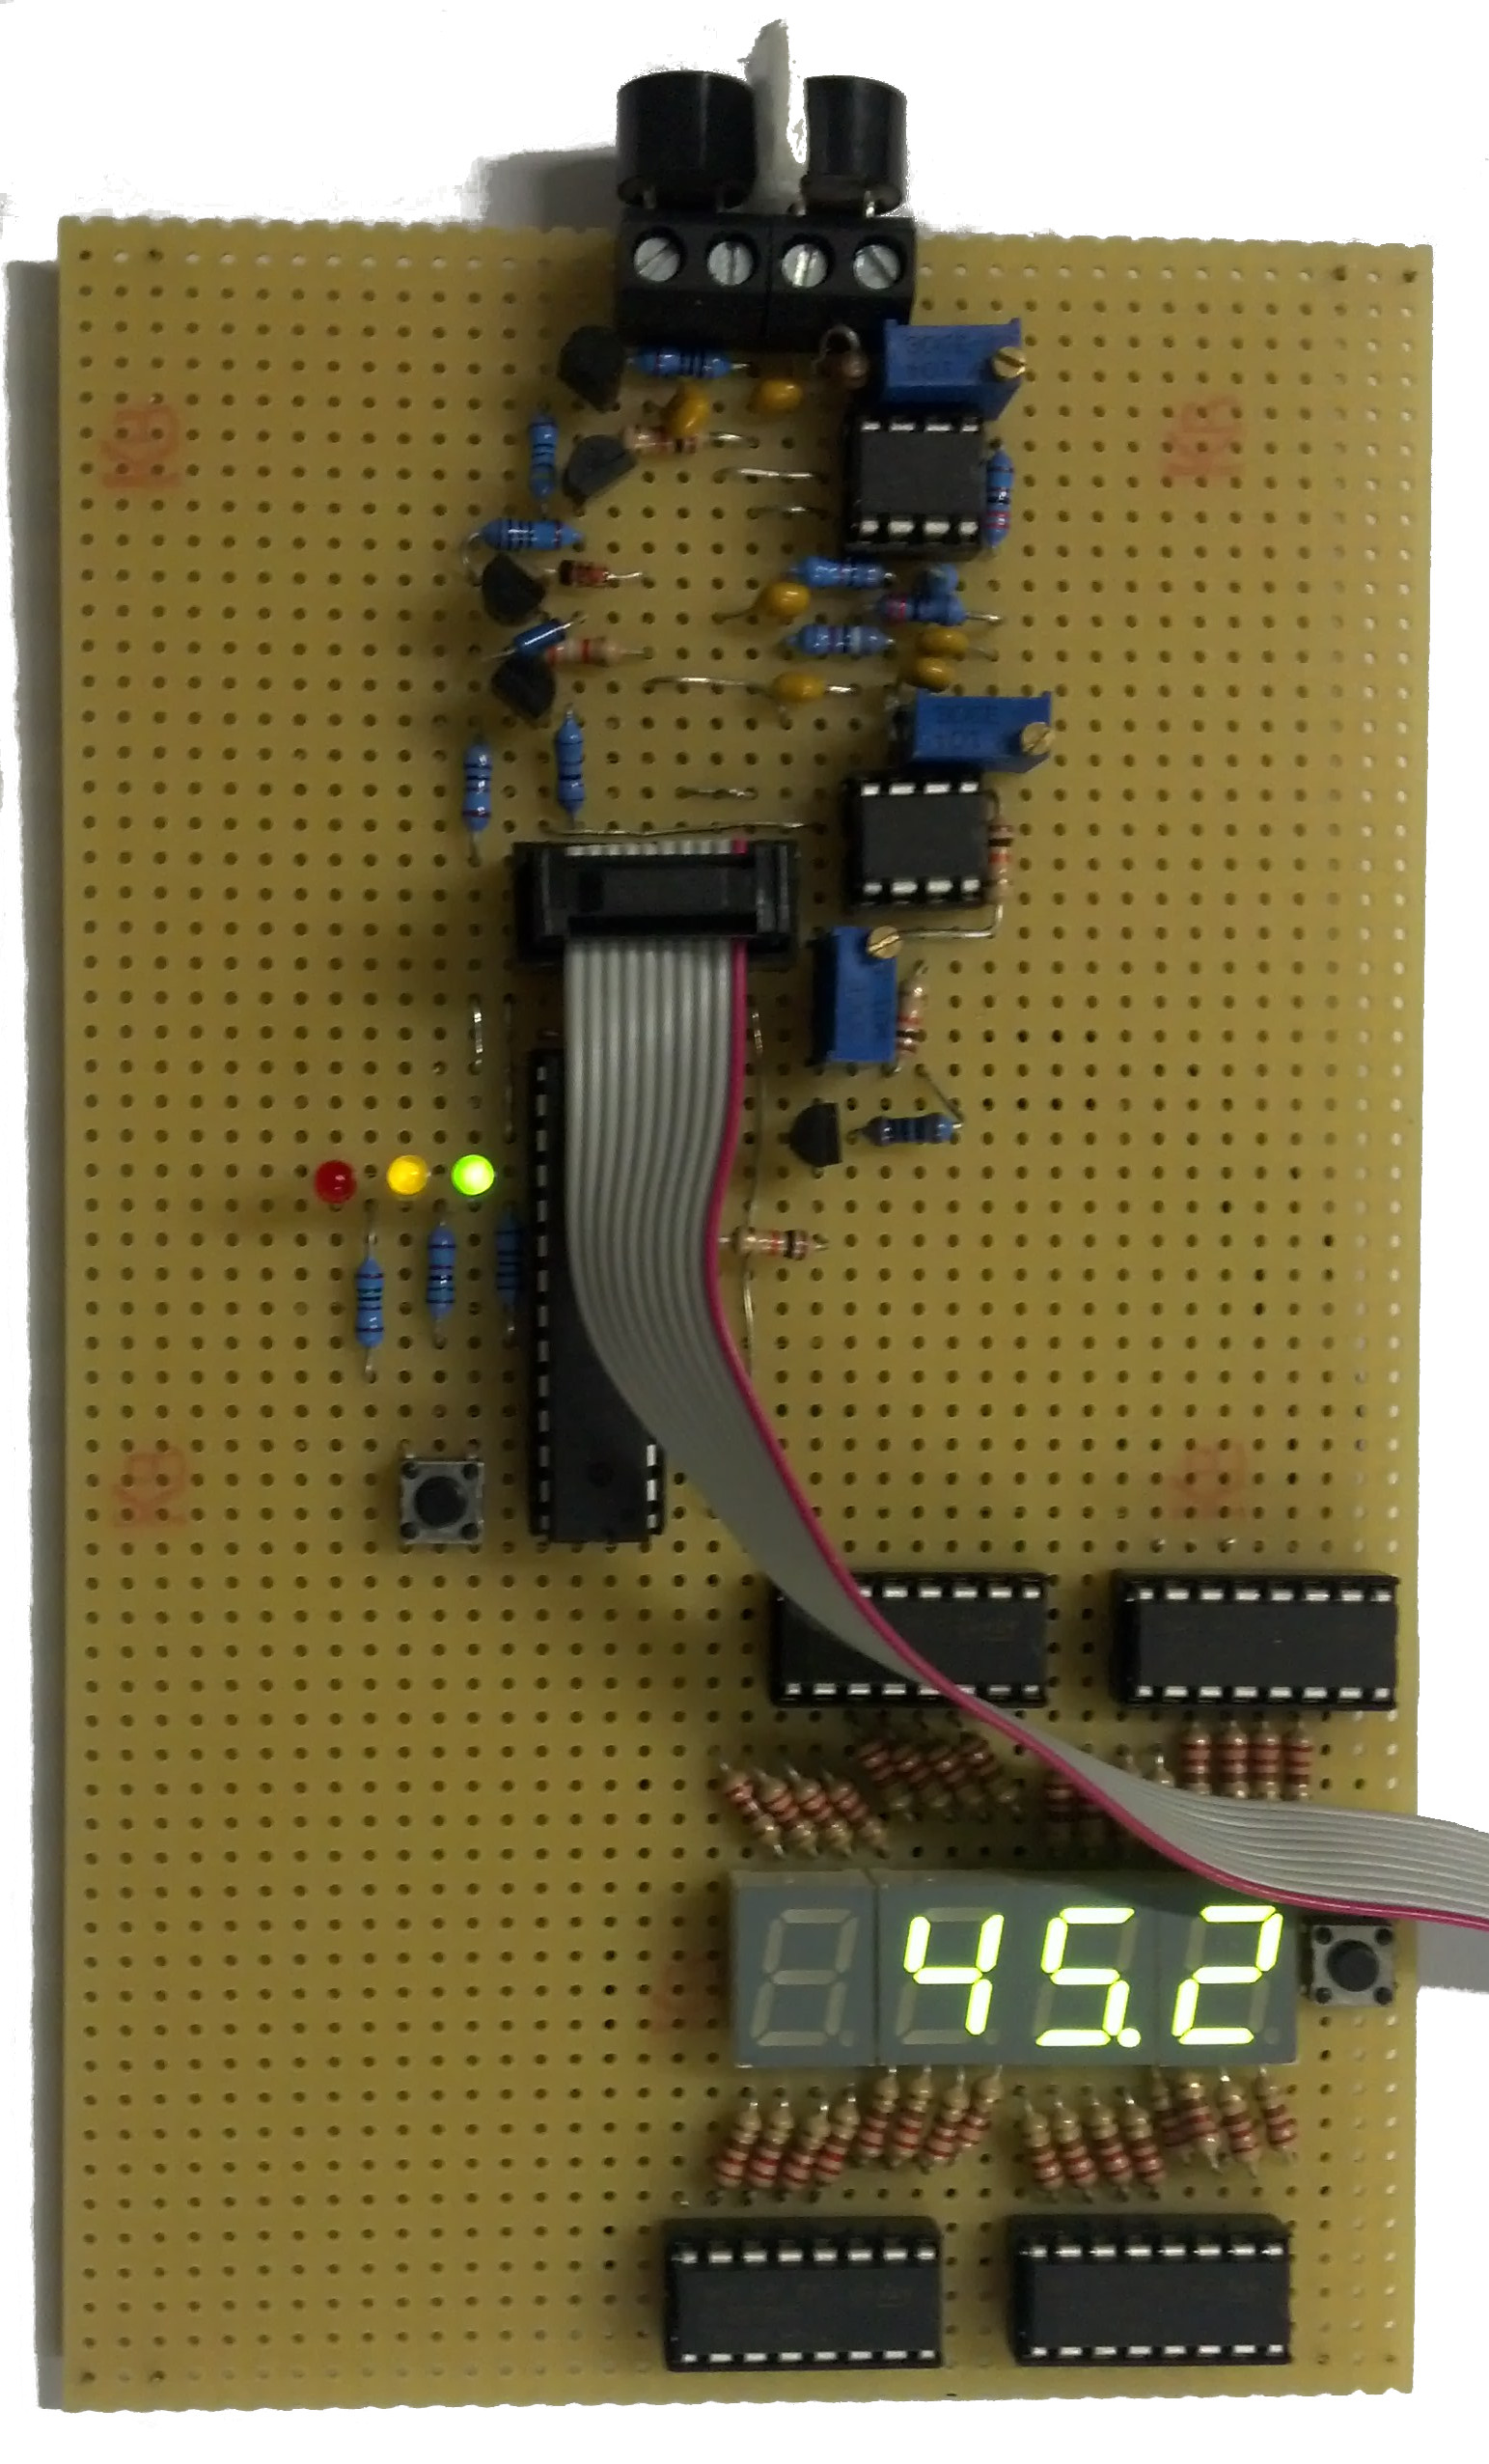
\includegraphics[width=(0.6\textwidth)]{fotos/platine.jpg}
	\caption{Prototyp-Platine mit Anzeige aus vier Ziffern} \label{img:prototype}
\end{figure}

\subsection{Aufbau}
Die Platine enthält die Sende- und Empfängerschaltung, den Mikrocontroller mit Anzeige-LEDs und Reset-Knopf, sowie eine Pfostenstecker-Buchse zur Verbindung mit der Verteilerplatine. Die Anzeige wurde nachträglich hinzugefügt. Obwohl der Platinenentwurf sehr platzsparend ist, wurde versucht die Schaltungen räumlich voneinander zu trennen. Dadurch können Wechselwirkungen verhindert werden.\\
Als Sendeschaltung ist die Gegentaktstufe (siehe \ref{schaltung:gegentakt}) zum Einsatz gekommen, da sie die leistungsfähigste Sendeschaltung ist und die höchste Reichweite verspricht. Die Empfangsschaltung wurde mit der Pulsverstärkung und Frequenzfilterung realisiert (\ref{schaltung:pulse}), da die Nachteile zu diesem Zeitpunkt noch nicht bekannt waren. Zudem sollte die Platine als Vorführobjekt auch Geschwindigkeiten über den Dopplereffekt messen können, dafür müssen die Pulse einzeln detektierbar sein.

\begin{figure}[H]
	\centering
	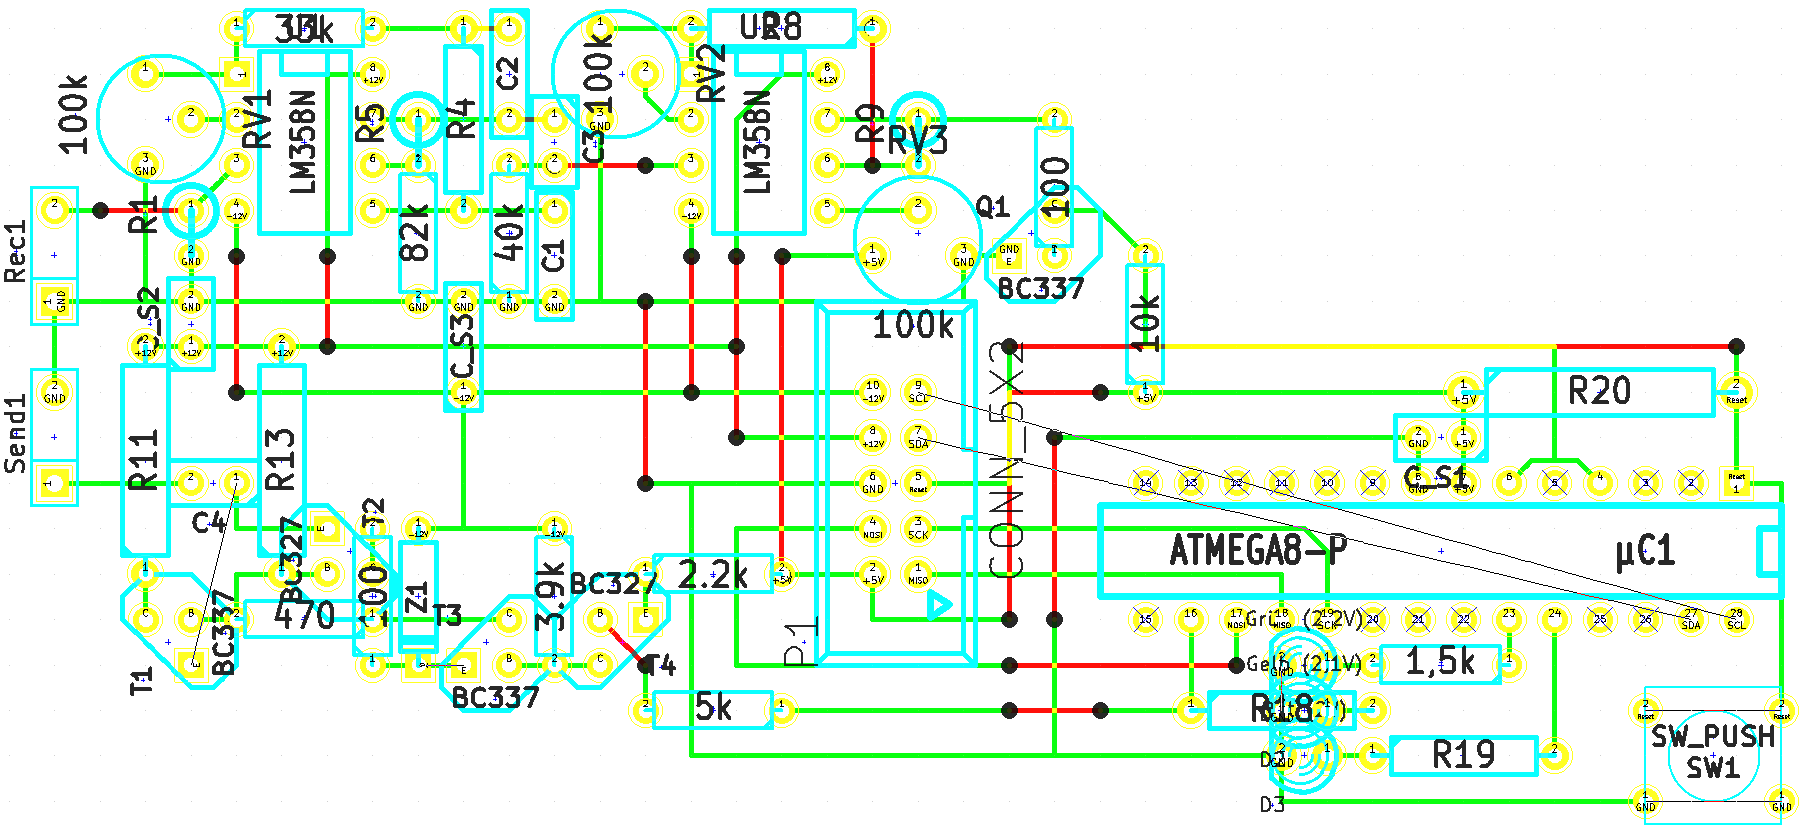
\includegraphics[width=(\textwidth)]{images/prototyp_2d.png}
	\caption{Platinenentwurf mit Sender, Empfänger und Mikrocontroller} \label{img:prototyp2d}
\end{figure}

\subsection{Probleme}
Das Löten des Platinenentwurfs stellte sich schwieriger heraus, als angenommen. Viele Komponenten wurden zu eng platziert, die Leiterbahnen waren zu verzweigt und es bestand die Gefahr eines Kurzschlusses. Außerdem wurden Sender und Empfänger zu nah aneinander platziert. Die Folge war, dass mechanische Schwingungen durch die Luft, aber auch über die Platine übertragen wurden. Abhilfe schaffte ein Stück Papier oder eine dünne Hartschaumplatte, die einen Großteil der Schwingungen reflektieren oder absorbiert. Eine Totzeit zwischen Senden und Empfangen ließ sich dennoch nicht vermeiden, sodass die minimal messbare Distanz bei ca. $15cm$ liegt. Auch elektrische Wechselwirkungen wurden festgestellt. Zusätzliche Abblock-Kondensatoren direkt an der Stromversorgung der ICs konnten die Effekte eindämmen.


\section{Sensorplatinen}
Die Sensorplatinen sind verkleinerte Versionen der Prototyp-Platine, wobei die Schaltungen durch die gesammelten Erkenntnisse verbessert und vereinfacht wurden. Anders als die Prototyp-Platine sind sie nicht mit einer Anzeige ausgestattet, sodass ein Betrieb ohne Kommunikationsverbindung per \ac{TWI} nicht möglich ist. Es gibt zwei Sensorplatinen, die zusammen mit der Prototyp-Platine für die Positionsbestimmung eingesetzt werden. Die Pinbelegung des Verbindungssteckers ist identisch mit der vorherigen Platine.

\begin{figure}[H]
	\centering
	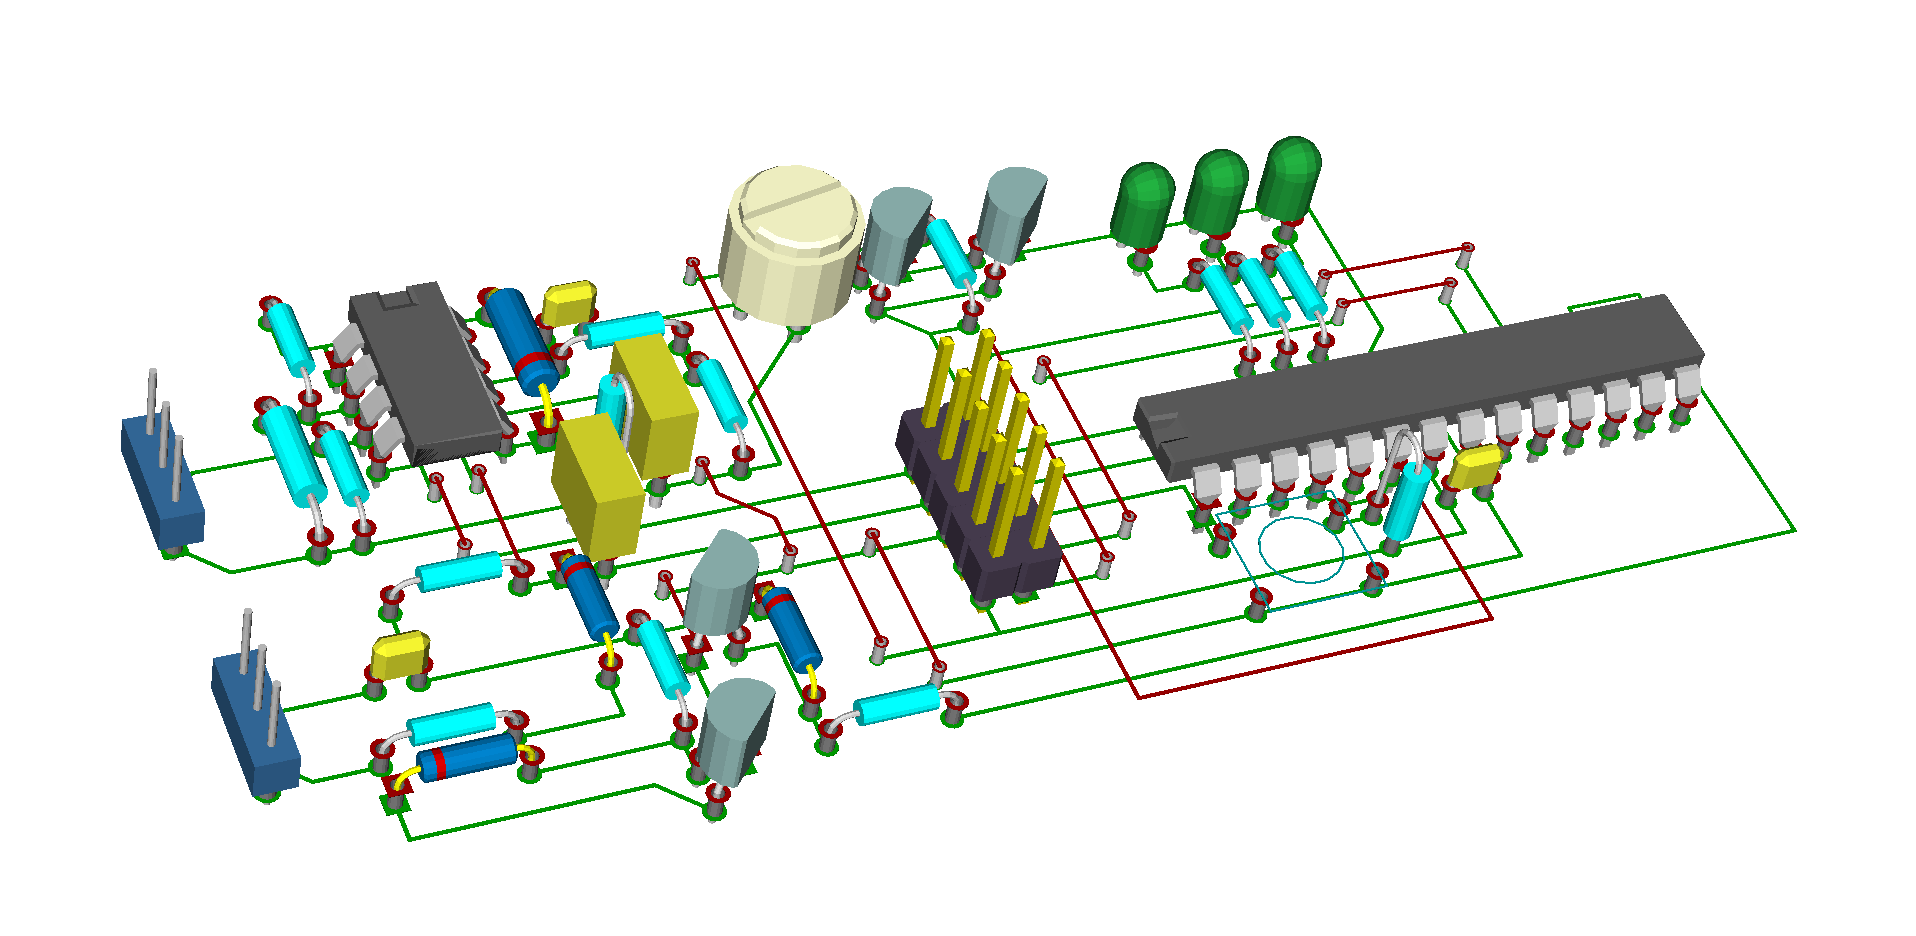
\includegraphics[width=(\textwidth)]{images/endplatine_3d.png}
	\caption{Platinenentwurf als 3D-Darstellung} \label{img:endplatine3d}
\end{figure}


\subsection{Änderungen der Schaltungen}
Die Gegentaktstufe als Sendeschaltung wurde durch eine einfache Transistor-Schaltung ersetzt, die ein Wechselsignal mit $20V$ Spannungsdifferenz erzeugt (siehe \ref{I:3}). Als Empfängerschaltung wurde der Integrierverstärker eingesetzt (\ref{schaltung:integrator}). Die Platine wurde durch die vereinfachten Schaltungen kompakter und erzielt ähnlich gute Ergebnisse wie die Prototyp-Platine.


\begin{figure}[H]
	\centering
	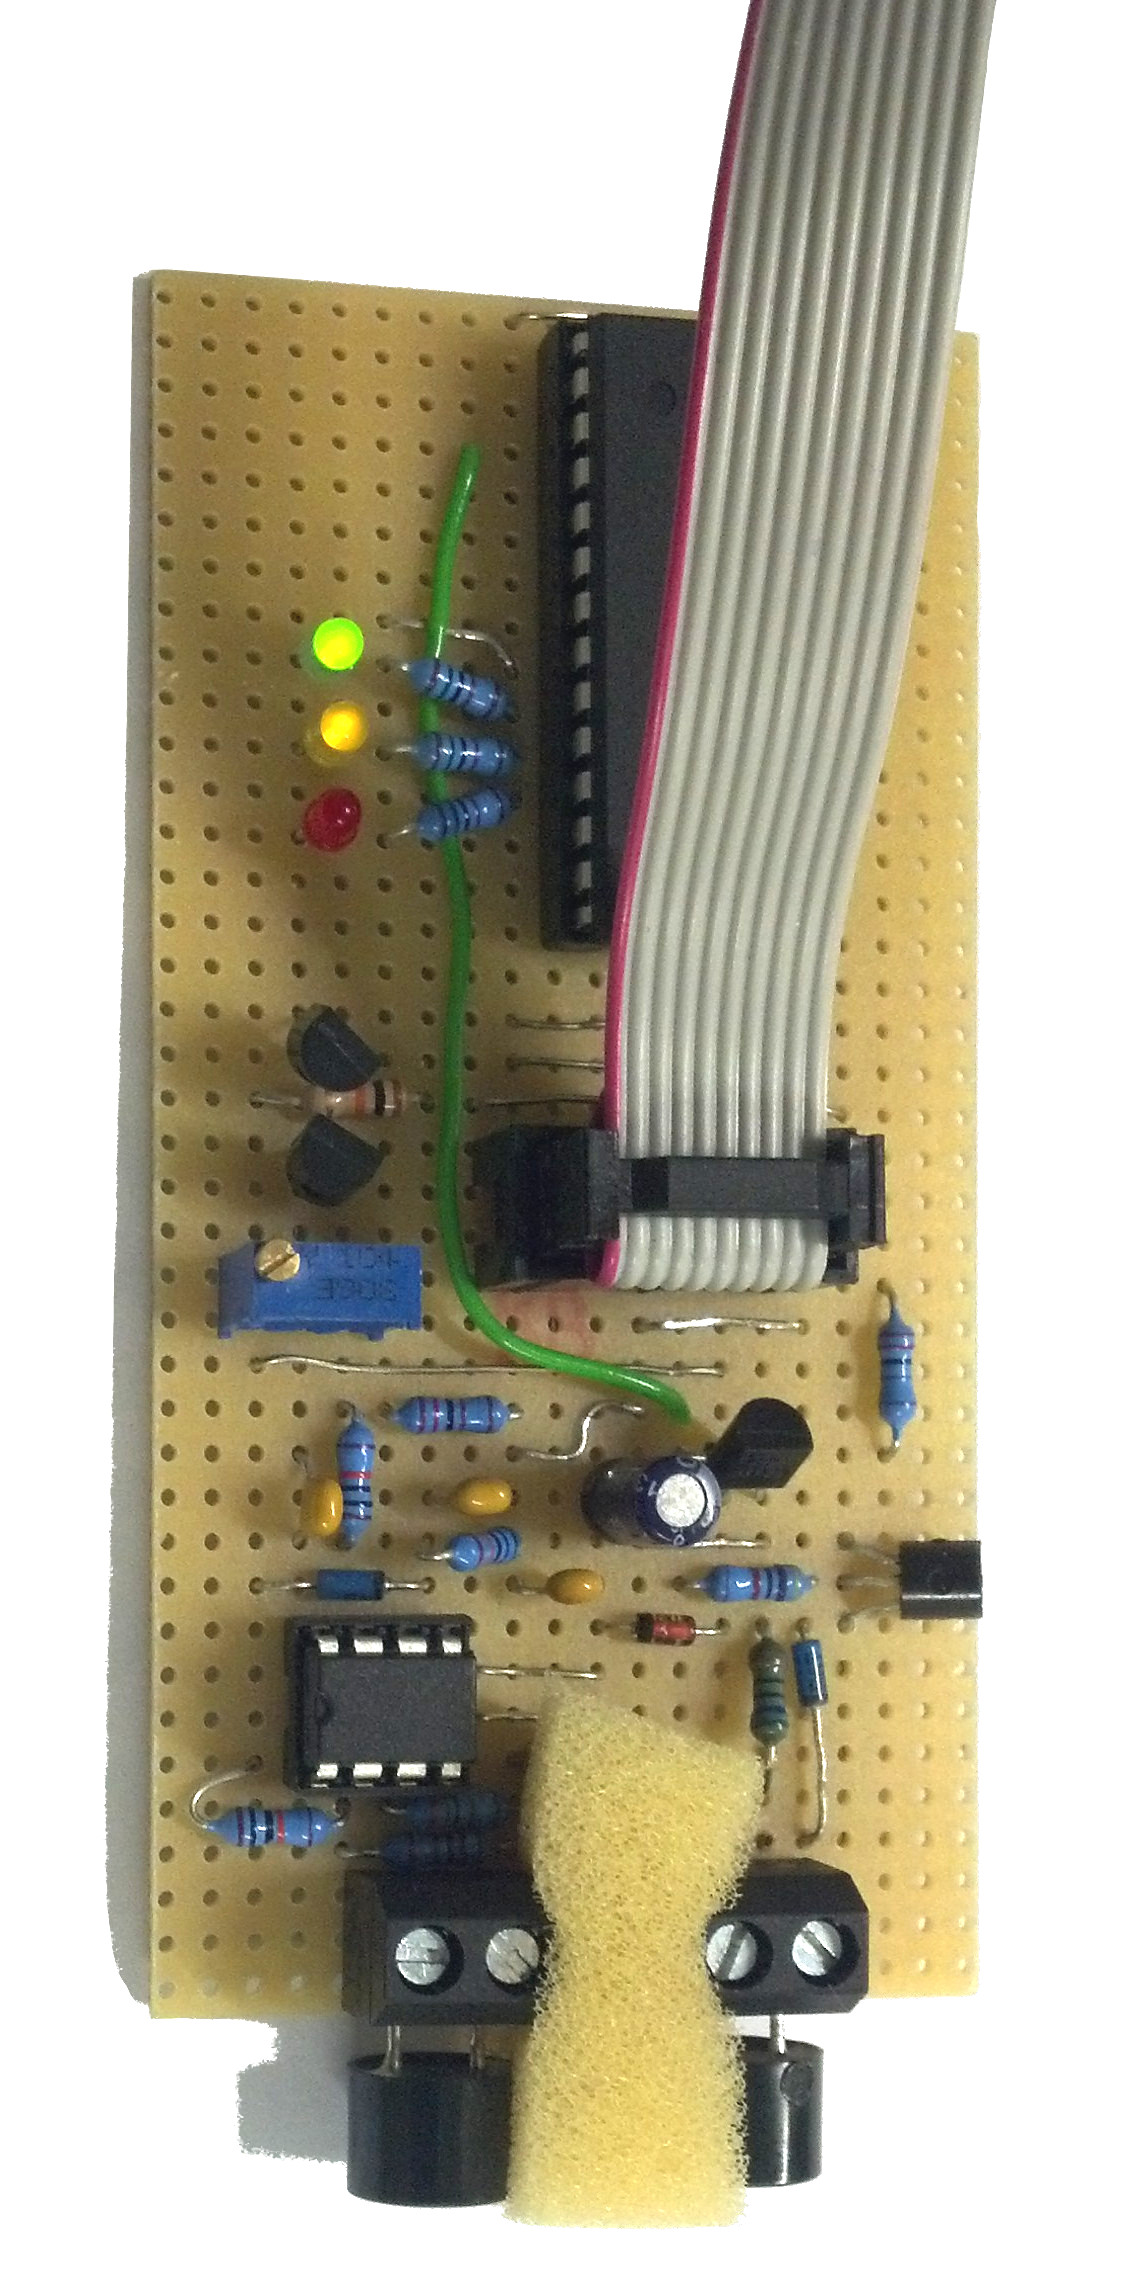
\includegraphics[angle=270, width=(\textwidth)]{fotos/platine_klein2.jpg}
	\caption{Fertige Sensorplatine} \label{img:endplatine_real}
\end{figure}

\subsection{Empfindlichkeit des Empfängers}
Durch die \textit{Darlington-Transistorschaltung} konnte eine hohe Empfindlichkeit am Empfänger erreicht werden. In einem Spezialfall führte das jedoch zu Problemen: Bei der Distanzmessung zwischen den Platinen werden Triggerimpulse über eine Leitung gesendet. Dieser Impuls koppelte geringe Störungen in die Stromversorgung ein, die bereits zum Durchschalten der Transistoren führten. Das Problem wurde gelöst, indem die Offsetspannung etwas geringer eingestellt wurde. Allerdings geht das zu Lasten der Reichweite der Sensoren, da die Signalpegel höher sein müssen, um die Transistoren zur richtigen Zeit durchschalten zu lassen.
\begin{figure}[H]
	\centering
	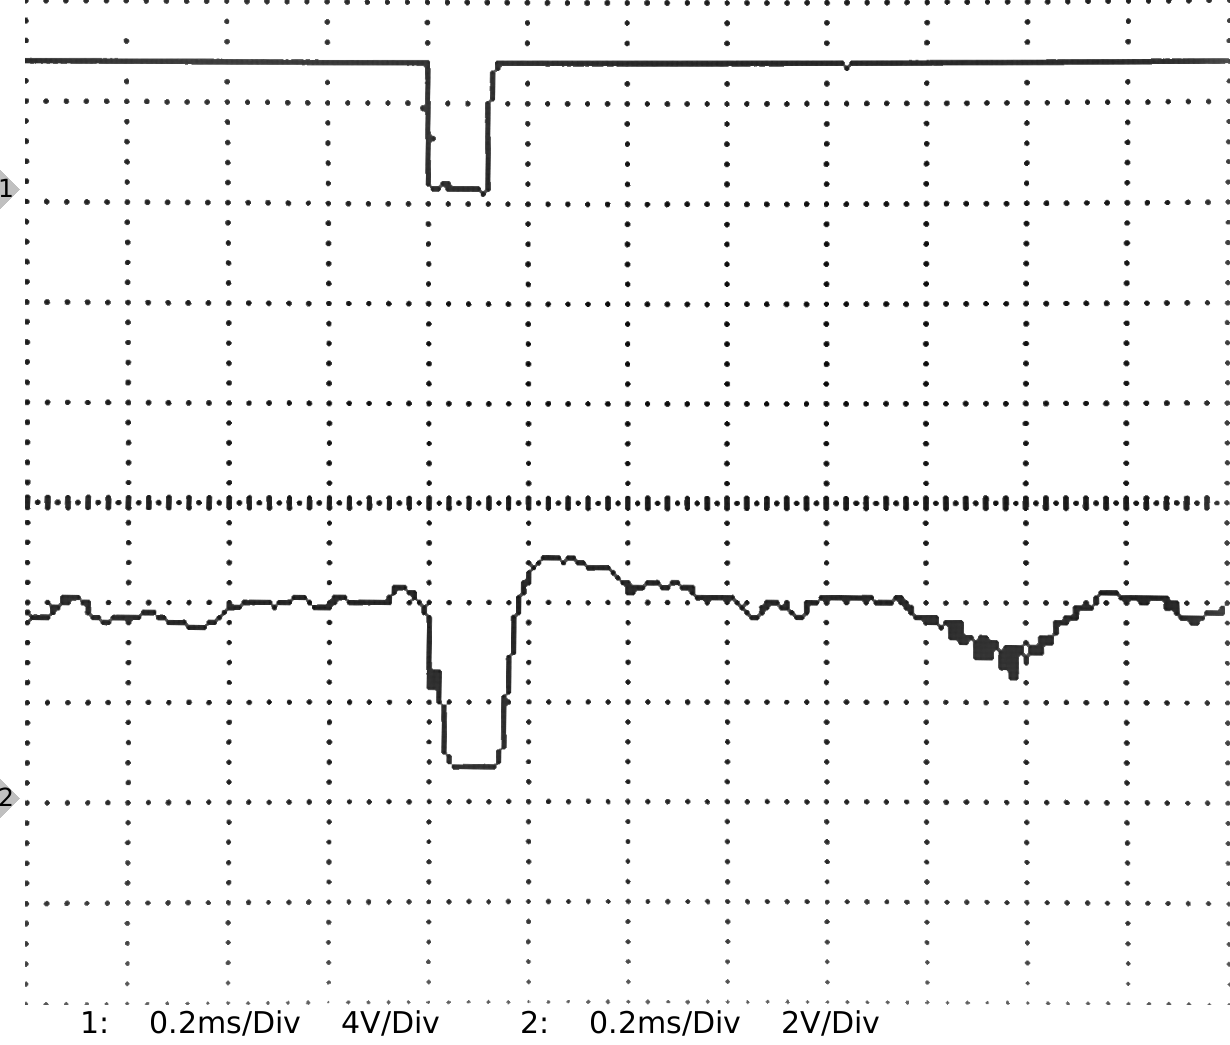
\includegraphics[width=(\textwidth)]{oszi/15-05-30/1.png}
	\caption{Empfindlich eingestellter Empfänger (unten) schaltet bei Trigger-Signal durch} \label{img:triggerimpuls}
\end{figure}


\section{Verteiler-Platine und Verkabelung}
Da der Verkabelungsaufwand durch die Stromversorgung und Kommunikationsschnittstellen relativ hoch ist, wurde zu Beginn entschlossen, eine zentrale Platine als Verteilungsglied zu verwenden. Die Platinen und der Computer werden über Flachbandkabel mit ihr verbunden, da sie stabil und kompakt sind. Zusätzlich wandelt die Platine einige Signalpegel, da das \ac{GPIO}-Interface des Raspberry Pi mit $3.3V$ arbeitet und nicht $5V$ tolerant ist, die AVR-Mikrocontroller jedoch mit $5V$ betrieben werden und den Computer beschädigen könnten. Die Platine besitzt auch einen Steckplatz, um die Mikrocontroller auf der Platine per \ac{ISP} programmieren zu können. Ursprünglich passierte dies über den Raspberry Pi, jedoch kam es zu einem Hardware-Defekt eines Pins, woraufhin ein externer ISP-Programmer zum Einsatz kam, der wiederum auf der Verteiler-Platine eingesteckt werden kann.\\
Die Pegelwandlung der \ac{TWI}-Schnittstelle erfolgt mit einem bidirektionalen Level-Shifter, der aus einem Mosfet-Transistor besteht. Er eignet sich für bidirektionale Kommunikationsverbindungen, die eine \textit{Open-Collector}-Ausgangsstufe benutzen. Über zwei Pullup-Widerstände werden die Pegel auf der jeweiligen Seite auf $3.3V$ und $5V$ gezogen. Das \textit{Gate} des Transistors ist mit $3.3V$ beschaltet, sodass höhere Spannungen von \textit{Drain} zu \textit{Source} abfallen und keine anderen Geräte beschädigen können. Der Pegel kann auf beiden Seiten auf \textit{Ground} gezogen werden. Da der Transistor leitfähig ist, kann das Signal passieren. %TODO: Quelle: http://www.hobbytronics.co.uk/mosfet-voltage-level-converter


